\documentclass[10pt,a4paper, nocenter]{report}
\usepackage[scaled=0.92]{helvet}
\usepackage[margin=1in]{geometry}
\usepackage[latin1]{inputenc}
\usepackage{blindtext}
\usepackage{amsmath}
\usepackage{appendix}
\usepackage{amsfonts}
\usepackage{amssymb,amsthm}
\usepackage{graphicx}
\usepackage{parskip}
\usepackage{fancyhdr}
\usepackage{lastpage}
\usepackage{enumerate,url}
\usepackage{etoolbox}
\usepackage{algorithm2e}
\usepackage{caption}
\usepackage{subcaption}

\makeatletter
\patchcmd{\chapter}{\if@openright\cleardoublepage\else\clearpage\fi}{}{}{}
\makeatother
\makeatletter
\patchcmd{\chapter}{\@maketitle\cleardoublepage}{}{}{}
\makeatother

\newtheorem{prop}{Proposition}
\newtheorem{theorem}{Theorem}
\newcommand{\abs}[1]{\lvert {#1} \rvert}
\newcommand{\norm}[1]{\lvert\lvert {#1} \rvert\rvert}


\pagestyle{fancy}
\lhead{[WORK IN PROGRESS] \\ Research Report - Spectral Clustering}
\rhead{Sourabh Antani}
\cfoot{\thepage\ of \pageref{LastPage}}
\renewcommand{\footrulewidth}{0.4pt}


\author{Sourabh Antani}
\title{[WORK IN PROGRESS] \\ Research Report - Spectral Clustering}
\date{}

\begin{document}
	\maketitle

	
	\chapter{Introduction}
    \thispagestyle{fancy}
    Nowadays, clustering has evolved into a class of most fundamental methods
    frequently applied in exploratory data analysis. Clustering helps the researchers understand the diversity of data and the number of different populations that exist. This knowledge, in turn, aids in subsequent tasks like the choice of modeling or classification techniques and the parameters for tuning them. 
	
    In this report, I will, first, list some of the commonly used clustering techniques before diving deeper into Spectral Clustering. In the next chapter, I will dig deeper into spectral clustering. Finally, I will list some of the possible avenues of research that I wish to explore. 

    \section*{Clustering Algorithms}
    Below are some examples of clustering algorithms used in practice, aside from spectral clustering. 
    
    Some common examples of algorithms that rely on euclidean distance and spatial density of points are:

    \begin{itemize}
        \item \textbf{$k$-means} This algorithm iteratively computes the centroids of the clusters using euclidean distances. The term was first used by J. Macqueen \cite{Macqueen67kmeans} but standard algorithm published by Lloyd \cite{Lloyd-82-kmeans}.
        \item \textbf{BIRCH (Balanced Iterative Reducing and Clustering using Hierarchies)} This algorithm extracts centroids from building hierarchies in height balance trees \cite{zhang-96-birch}
        \item \textbf{Mean-shift} This algorithm initializes the centroids randomly but then iteratively refines them by updating the centroids to be the centroid of all the points in a neighborhood of each of them \cite{Cheng95meanshift}.
        \item \textbf{DBSCAN} This algorithm creates clusters by looking at the density of a neighborhood of a point and combining nearby areas density equal to or higher than a given threshold \cite{Ester96adensity-based}
    \end{itemize}
        While these are generally simpler to understand, the 'shape' of the spatial distribution greatly affects the effectiveness of these algorithms. 

    Some examples of algorithms based on linear algebra/matrix factorization are:
    \begin{itemize}
        \item \textbf{Non-Negative Matrix Factorization} The main idea of this algorithm is to express a large matrix as the product of a tall and a wide matrix. The columns of the tall matrix represent the centroids of the clusters. The columns of the input matrix can be computed as a linear combination of the columns of the tall matrix with the coefficients from a column of the wide matrix \cite{Lawton-1971-nnmf} \cite{Paatero1991-nnmf}. Later \cite{Ding05-nnmf-spectral} studied the equivalence of NNMF with Spectral Clustering. This technique seeks to factorize the matrix and use one of the factors as the approximate basis for the matrix, thus effectively reducing the dimensionality of the problem. Another advantage of these methods is that it simple to gauge how 'good' the approximation is by looking at the difference between the product of approximated factors and the original matrix.
        \item \textbf{PCA Based clustering} The idea of this method is to apply PCA to a dataset and then plot the data on the first two principal components and apply $k$-means clustering. \cite{Zhang-2108-pca} 
    \end{itemize}

    


    \chapter{Spectral Clustering}
    An excellent tutorial for Spectral Clustering can be found in \cite{Luxburg2007}. Before we look at the various algorithms, let us go through some basic terms involved.

    \section{Some Terminology}

        Given an \textbf{undirected graph} $\mathbf{G=(V,E)}$ with $\mathbf{V=\{v_{1},\dots,v_{n}\}}$ being the \textbf{set of vertices} and $\mathbf{E}$ being the \textbf{set of weighted edges} such that each edge between two vertices $v_{i}$ and $v_{j}$ carries a non-negative weight $w_{ij} \ge 0$.

        The \textbf{Weighted \textit{adjacency matrix}} of the graph is the matrix $\mathbf{W=(w_{ij})_{i,j=1,\dots,n}}$. If $w_{ij}=0$, vertices $v_{i}$ and $v_{j}$ are not connected. $w_{ij}=w_{ji}$ since $G$ is undirected. 

        The \textbf{degree of a vertex} $v_{i}\in V$ is defined as $ \mathbf{d_{i} = \sum_{j=1}^{n}w_{ij}}$. \textbf{\textit{Degree matrix}} $\mathbf{D}$ is defined as the diagonal matrix with the degrees $d_{1} ,\dots, d_{n}$ on the diagonal. 

        $\mathbf{\bar{A}}$ denotes the \textbf{Complement} $V \backslash A$  of a given subset $A \subset V$. \textbf{Indicator vector} $\mathbf{1}_{A}$ is a vector with entries $f_{i} = 1$ if $v_{i} \in A$, $f_{i}=0$ otherwise.

        Define $\mathbf{W(A,B) = \sum_{i\in A, j\in B}w_{ij}}$, for not necessarily disjoint sets $A, B \subset V$.
        The \textbf{'size'} of $A \subset V$ can be measured in two ways, $\mathbf{\lvert A \rvert}$ := \textbf{number of vertices in $A$} or $\mathbf{vol(A)}$ := $\mathbf{\sum_{i\in A}d_{i}}$ which is \textbf{the sum of edge weights} attached to the vertices in $A$

        A subset $A \subset V$ of a graph is \textbf{connected} if any two vertices in $A$ can be joined by a path such that all intermediate points also lie in $A$. $A$ is called \textbf{Connected Component} if it is a connected subset such that $A$ and $\bar{A}$ are disjoint. Finally, \textbf{Partitions} of a graph are defined as non-empty sets $A_{1},\dots,A_{k}$ form partition of graph if $A_{i} \cap A_{j} = \emptyset$ and $A_{1}\cup \dots \cup A_{k} = V$

    \section{Graph Laplacians and Graph cuts}
    \subsection{Graph Laplacians}
        The following types of graph Laplacians have been defined in the literature:
        \begin{align*}
         \textbf{Unnormalized Graph Laplacian: } &L = D- W \\
         \textbf{Normalized Graph Laplacian (Symmetric): } &L_{sym} = D^{-1/2}LD^{-1/2} = I - D^{-1/2}WD^{-1/2} \\
         \textbf{Normalized Graph Laplacian (Random walk): } &L_{rw} = D^{-1}L = I - D^{-1}W 
        \end{align*}

		Below are some important properties of the three graph Laplacians:
		\begin{itemize}
			\item All three graph Laplacians are positive-semidefinte and have non-negative real-valued eigenvalues.
			\item 0 is an eigenvalue with multiplicity equal to the number of connected components of the graph. Thus for a fully connected graph one of the eigenvalues is 0. \item $L$ and $L_{sym}$ are symmetric. 
			\item The eigenvectors of $L_{rw}$ are the eigenvectors of $L$ while $D^{1/2}u$ is eigenvector of $L_{sym}$ if $u$ is eigenvector of $L$. 
        
    	\end{itemize}
    For proofs of the above properties, refer to the appendix. As far as naming goes, $L_{sym}$ follows from its structure. While $L_{rw}$ is so named because its structure is derived from the point of view of random walk on the graph. Taking $p_j = w_{ij}/d_i$ as the probability of an edge between $v_i$ and $v_j$ being selected for random walk, the transition matrix for the random walk is defined by $P = D^{-1}W$. Thus $L_{rw} = I-P$. This is why the second form of normalized graph Laplacian is denoted by $L_{rw}$.
    
    For information about unnormalized graph Laplacian, refer to \cite{mohar-1991} and \cite{mohar-1997} while the standard reference for normalized graph Laplacian is \cite{graph-spectral-book}. Formal equivalence between Ncut and transition probability of the random walk has been outlined in \cite{Meila01arandom}

    \subsection{Graph Cuts}
        The intuition of clustering is to divide the graph into groups of vertices such that the edges between the vertices in the same group have high weight and the edges between vertices from different groups have zero or very low weight. Thus effective clustering is to solve the minicut problem which can be defined as, for a given number $k$ subsets, choosing the partition $A_{1}, \dots, A_{k}$ which minimizes $$ \text{cut}(A_{1}, \dots, A_{k}) := \frac{1}{2}\sum_{i-1}^{k}W(A_i,\bar{A}_{i}) $$

        To reduce the chances that minicut simply separates an individual vertex, two approaches have been suggested to make sure that the clusters are 'reasonably large'. 

        First is RatioCut \cite{hagen-kahng-1992} where the solution is to solve minicut problem while dividing the graph in components with roughly the same number of vertices. The second approach is Ncut \cite{Shi-Malik-maxcut-00} which tries to solve the minicut problem by keeping the volume of each component, i.e. sum of edge weights, roughly the same.
        
        Thus, the objective functions that we seek to minimize are
        \begin{align*}
            RatioCut(A_{1},\dots,A_{k}) &= \frac{1}{2} \sum_{i=1}^{k}\frac{W(A_{i},\bar{A}_{i})}{\lvert A_{i} \rvert}
            = \sum_{i=1}^{k}\frac{cut(A_{i},\bar{A}_{i})}{\lvert A_{i} \rvert} \\
            Ncut(A_{1},\dots,A_{k}) &= \frac{1}{2}\sum_{i=1}^{k}\frac{W(A_{i},\bar{A}_{i})}{vol(A_{i})} = 
            \sum_{i=1}^{k}\frac{cut(A_{i},\bar{A}_{i})}{vol(A_{i})}
        \end{align*}
    
        While the introduction of these balancing condition makes the mincut problem NP-hard, relaxing these conditions slightly leads Ncut and RatioCut to normalized and unnormalized spectral clustering respectively \cite{Luxburg2007}

    \subsection{Perturbation theory point of view}
        Perturbation theory states that the eigenvalues and eigenvectors of a matrix $A$ and a perturbed matrix $A+H$ is bounded by a constant times the norm of $H$. To apply this to spectral clustering, consider the ideal case where the graph is composed by $k$  connected components. In this case, the first $k$ eigenvalues will be 0 and corresponding eigenvectors will be the indicator vector of the cluster, where exactly one entry (corresponding to the cluster) will be 1 and rest will be 0. In this case, $k$-means will trivially converge to the indicator vectors and clustering will be ideal. With a small perturbation, the eigenvectors will also be slightly perturbed but $k$-means should still converge to the correct centroids. However, if the noise or perturbation is large, or the non-zero eigenvalues are very close to 0 or eigengap is very small, thus producing eigenvectors whose original values are very close to 0, the perturbation may be large enough for $k$-means to predictably converge to the correct centroids. The problem mentioned in the last section is not common for $L$ or $L_{rw}$ but for $L_{sym}$ the eigenvectors are already left multiplied by $D^{1/2}$ and can cause trouble. Hence the third algorithm below \cite{ng-jordan-01} needs an extra normalization step. 

    \section{Algorithms}

    Three classic spectral clustering algorithms can be found in literature.

    All three algorithms essentially follow the same steps, using the first $k$ eigenvectors of the graph Laplacian, create a matrix and then create $k$ clusters from the rows of that matrix using k-Means algorithm. Finally, create the clusters of data points with the same indices as the indices of the matrix rows in the $k$ clusters formed by k-means. For a proof of how the relaxation of the above balancing conditions to arrive at an approximation of NCut and RatioCut leads to the Normalized and Unnormalized Spectral Clustering respectively, see \cite{Luxburg2007}
	
	\subsection{Unnormalized Spectral Clustering}
    \begin{algorithm}
        \DontPrintSemicolon
        \KwIn{Similarity matrix $S \in \mathbb{R}^{n\times n}$, number $k$ of clusters to construct.}
        \Begin{
		Construct a similarity graph and its weighted adjacency matrix $W$\;
		Compute the unnormalized Laplacian $L$\;
		Compute the first $k$ eigenvectors $u_{1},\dots, u_{k} $ of $L$\;
		Let $U \in \mathbb{R}^{n\times k}$ be the matrix containing the vectors $u_{1},\dots, u_{k}$ as columns\;
		For $i = 1,\dots, n$, let $y_{i} \in \mathbb{R}^k$ be the vector corresponding to the $i^{th}$ row of $U$\;
		 Cluster the points $(y_{i}), i=1,\dots,n$ in $\mathbb{R}^k$ with the k-means algorithm into clusters
		$C_{1},\dots, C_{k}$\;}
        \KwOut{Clusters $A_{1},\dots, A_{k}$ with $A_{i} = \{x_{j}| y_{j} \in C_{i}\}$}
    \end{algorithm}

	\subsection{Normalized Spectral Clustering - Shi \& Malik (2000)\cite{Shi-Malik-maxcut-00}}
	\textit{This algorithm uses generalized eigenvectors of L, which are the eigenvectors of normalized random-walk Laplacian $L_{rw}$}
    \begin{algorithm}
        \DontPrintSemicolon
        \KwIn{Similarity matrix $S \in \mathbb{R}^{n\times n}$, number $k$ of clusters to construct}
	    \Begin{
            Construct a similarity graph and its weighted adjacency matrix $W$\;
            Compute the unnormalized Laplacian $L$.\;
            Compute the first $k$ generalized eigenvectors $u_{1},\dots, u_{k} $ of generalized eigenproblem $Lu = \lambda Du$.\;
            Let $U \in \mathbb{R}^{n\times k}$ be the matrix containing the vectors $u_{1},\dots, u_{k}$ as columns.\;
            For $i = 1,\dots, n$, let $y_{i} \in \mathbb{R}^k$ be the vector corresponding to the $i^{th}$ row of $U$.\;
            Cluster the points $(y_{i}), i=1,\dots,n$ in $\mathbb{R}^k$ with the k-means algorithm into clusters $C_{1},\dots, C_{k}$.\;
	    }
	    \KwOut{Clusters $A_{1},\dots, A_{k}$ with $A_{i} = \{x_{j}| y_{j} \in C_{i}\}$}
    \end{algorithm}

    \subsection{Normalized Spectral Clustering - Ng, Jordan \& Weiss (2002)\cite{ng-jordan-01}}
	\textit{This algorithm uses the eigenvectors of normalized symmetric Laplacian $L_{sym}$. Note that if $D^{1/2}u$ is an eigenvector of $L_{sym}$ if $u$ is an eigenvector of $L$ hence an additional normalization step is needed.}

	\begin{algorithm}[H]
        \DontPrintSemicolon
        \KwIn{Similarity matrix $S \in \mathbb{R}^{n\times n}$, number $k$ of clusters to construct.}
        \Begin{
            Construct a similarity graph and its weighted adjacency matrix $W$\;
            Compute the normalized Laplacian $L_{sym}$\;
            Compute the first $k$ eigenvectors $u_{1},\dots, u_{k} $ of $L_{sym}$\;
            Let $U \in \mathbb{R}^{n\times k}$ be the matrix containing the vectors $u_{1},\dots, u_{k}$ as columns\;
            Form the matrix $T \in \mathbb{R}^{n\times k}$ from $U$ by normalizing the norm to 1, $t_{ij} = u_{ij}/(\sum_{k}u_{ik}^2)^{1/2}$\;
            For $i = 1,\dots, n$, let $y_{i} \in \mathbb{R}^k$ be the vector corresponding to the $i^{th}$ row of $U$\;
            Cluster the points $(y_{i}), i=1,\dots,n$ in $\mathbb{R}^k$ with the k-means algorithm into clusters $C_{1},\dots, C_{k}$\;
        } 
        \KwOut{Clusters $A_{1},\dots, A_{k}$ with $A_{i} = \{x_{j}| y_{j} \in C_{i}\}$}
    \end{algorithm}

    \subsection{Numerical Experiments}

    Using my implementation of the above algorithms, here are some results of my experiments

    \begin{enumerate}
        \item{Mixture of 4 Gaussians in $\mathbb{R}^1$}\\
        This data set consists of a random sample of 200 points drawn according to a mixture of four Gaussians. The similarity function used was a Gaussian kernel $e^{-\abs{x_i - x_j}^2/(2\sigma^2)}$ with $\sigma = 1$. The distribution of points, pictorial representation of matrices $W$ and $D$, and the final clustering results are shown in Figure \ref{fig:1dresults}

        \begin{figure}[h]
        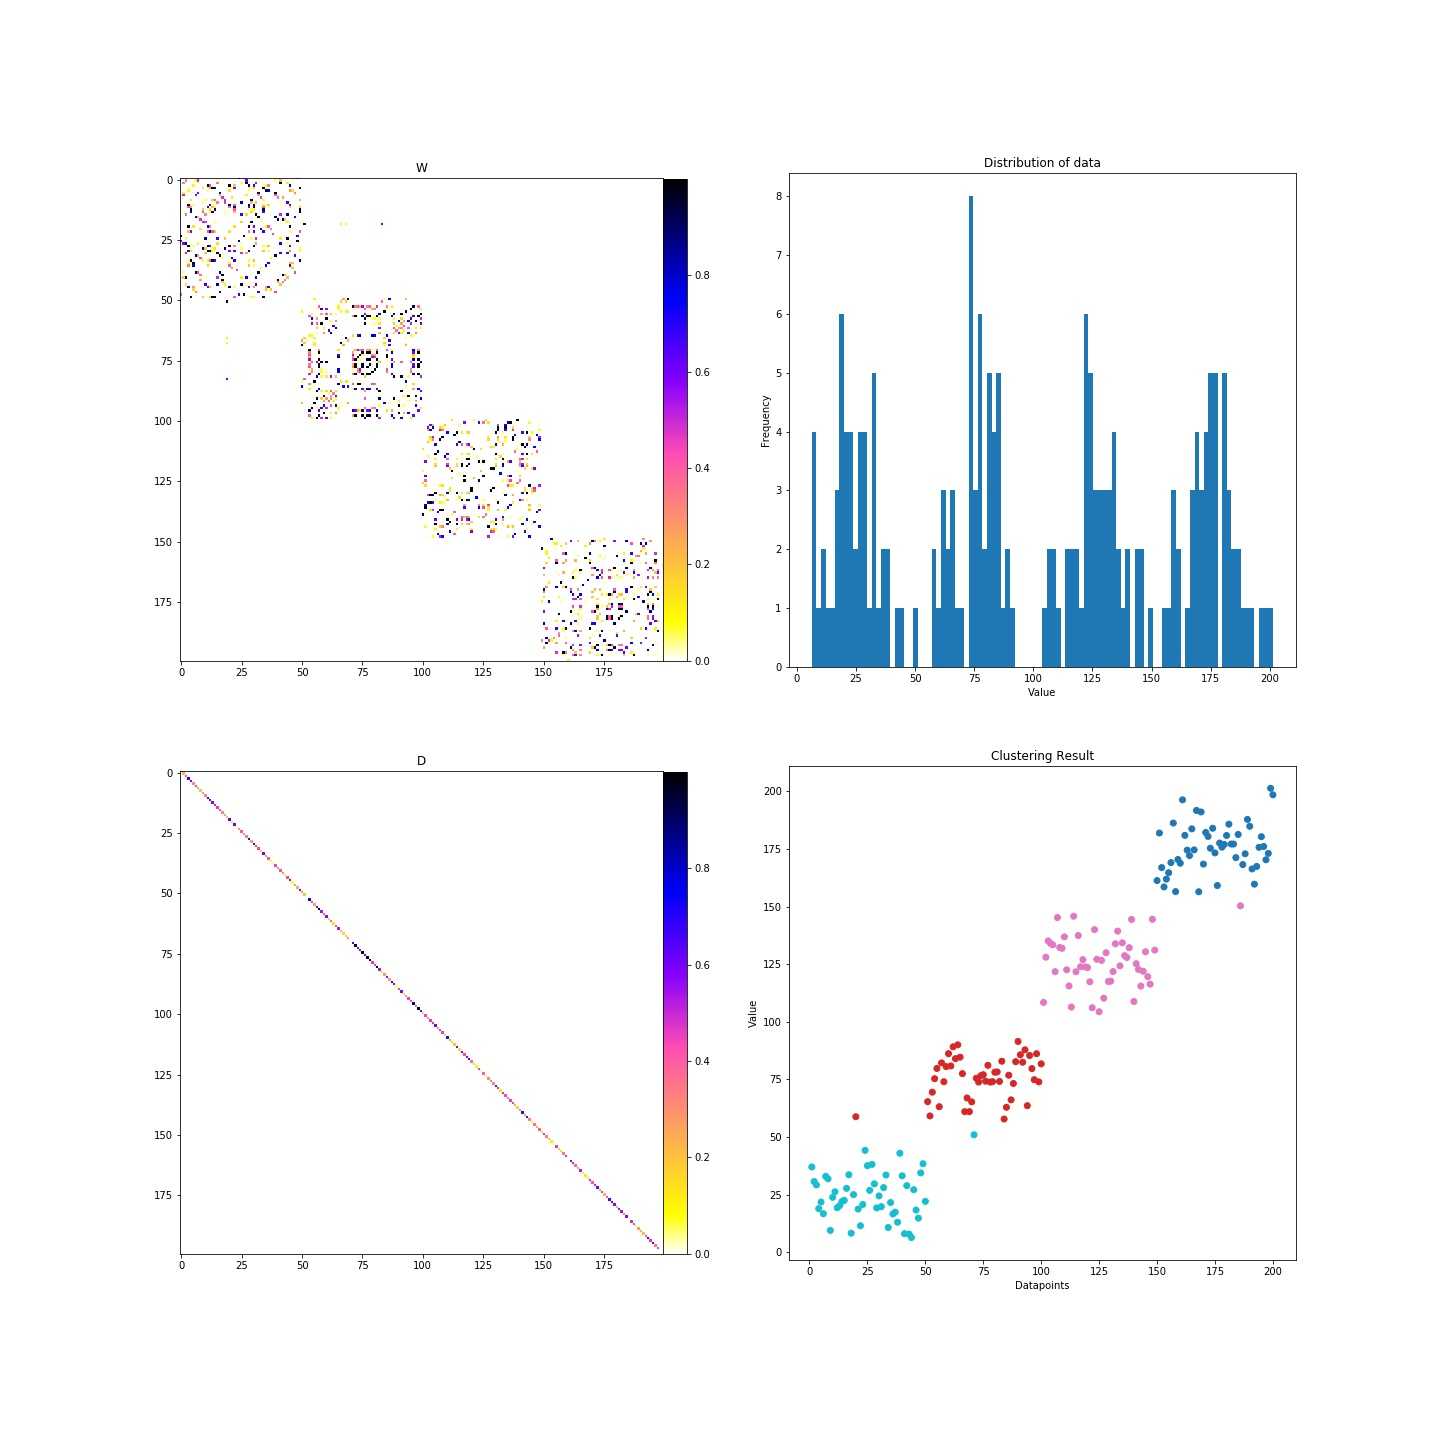
\includegraphics[width=0.9\textwidth]{../../images/1DCluster.jpg}
        \caption{Clustering results for 200 points in $\mathbb{R}^1$}
        \label{fig:1dresults}
        \end{figure}

        \item{Points in $\mathbb{R}^2$}\\
        This data set (the 'dim2' dataset from \cite{DIMLow}) consists of 1351 points in $\mathbb{R}^2$ distributed in 9 clusters with one outlier. The figure below shows the clustering in 5, 8, and 10 clusters. This example shows that even though in theory, both Ncut and RatioCut try to keep the clusters reasonably large, that if a single outlier point would be clustered independently if it is sufficiently separated from the rest. The reason for this is that rest of the clusters are very tightly organized. The similarity function used in this case was scaled Euclidean distance. The clustering results into 5, 8, and 10 clusters is shown in Figure \ref{fig:2dresults}
        \begin{figure}[h]
        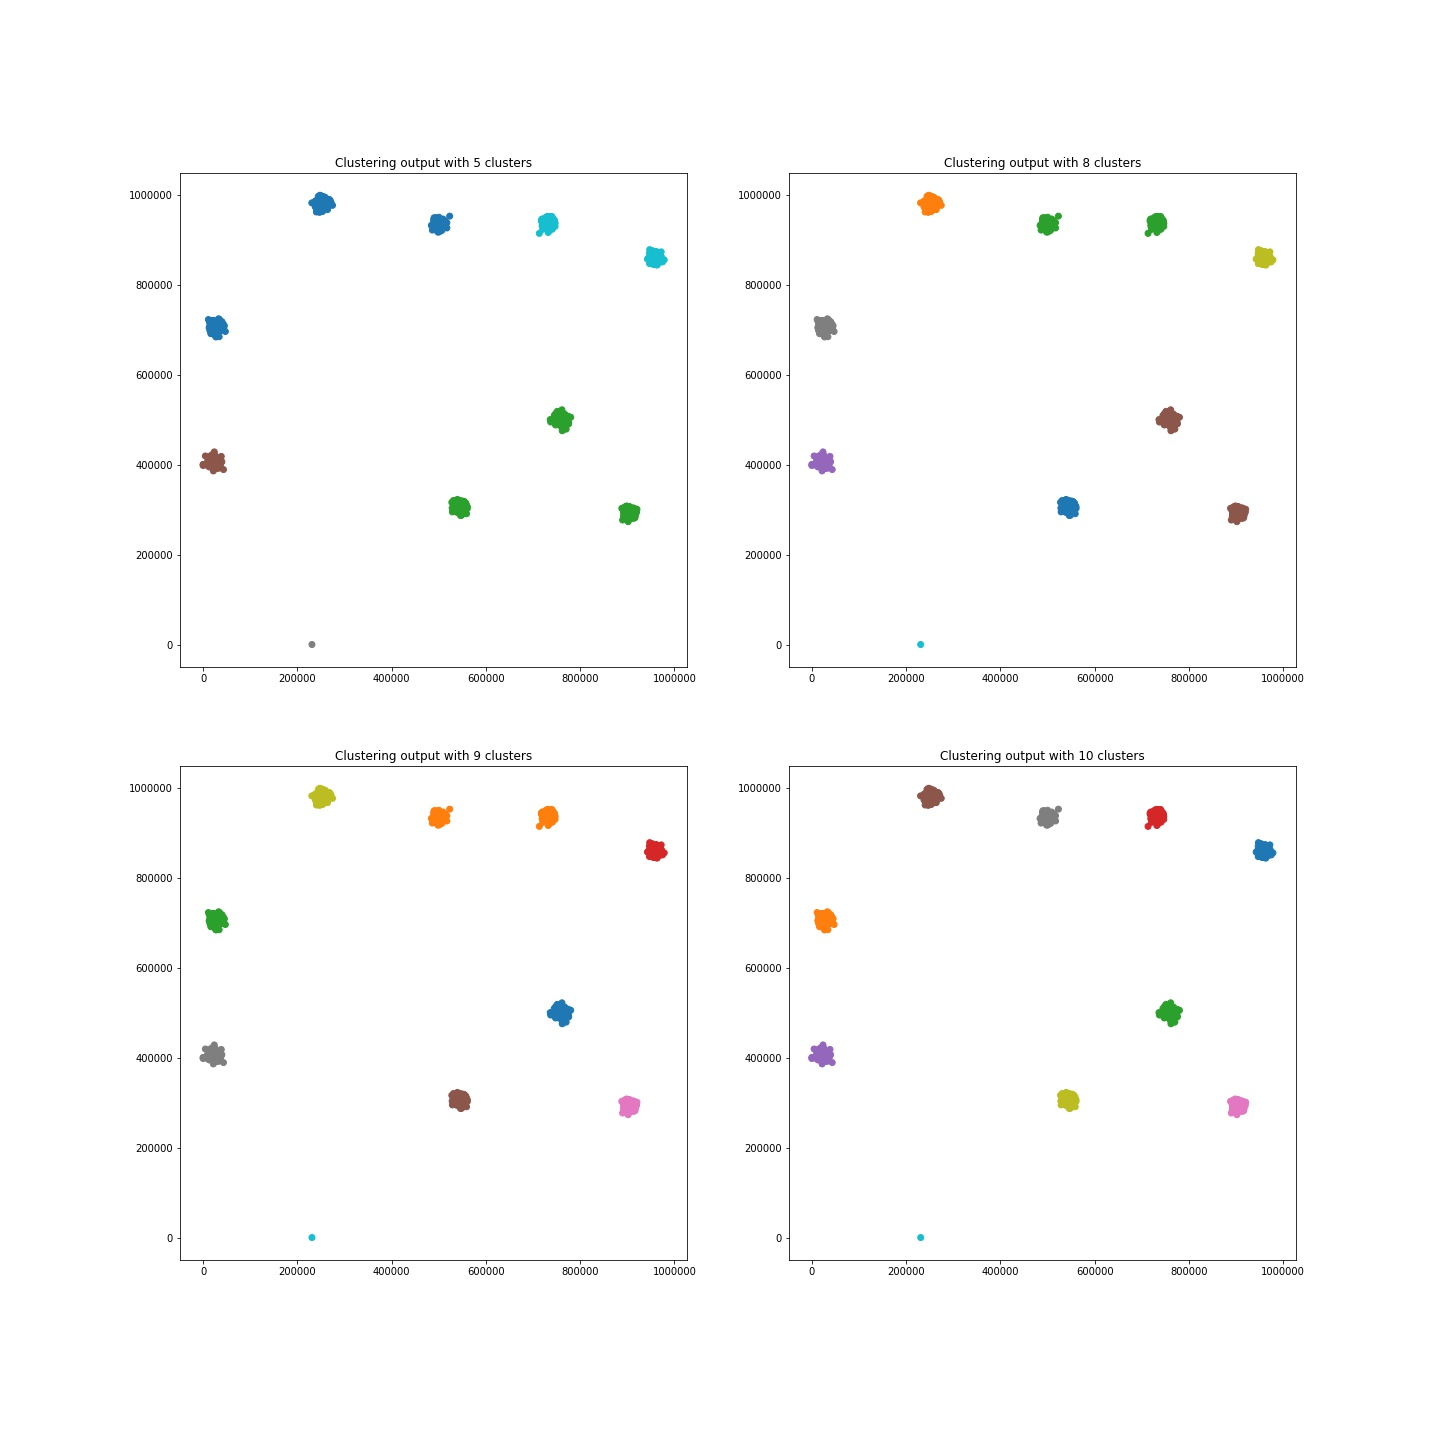
\includegraphics[width=\textwidth]{../../images/2DCluster.jpg}
        \caption{Clustering results for 1351 points in $\mathbb{R}^2$}
        \label{fig:2dresults}
        \end{figure}

        \item{Unsupervised Image Classification}\\
        Image recognition is generally considered to be a supervised machine learning problem. A trained neural network can recognize and classify images with very high accuracy. However, this requires that the training set images need to be labeled. One such application arises in biology and medical imaging and manually labeling the training set of images may not be possible since trained personnel would be required for the purpose. One way to handle this type of situation is to cluster these images and then inspect a small sample of images from each cluster. If clustering was effective, the images in a cluster generally would fall under one category (in this case, the same digit) and the manual task gets reduced to labeling the cluster. To test this approach, I took 2000 images from the MNIST dataset. The MNIST dataset is a set of images of handwritten digits and each image is a 28$\times$28-pixel single color image converted to an array of 784 (28 $\times$ 28) integers from 0 to 256 representing the intensity of the color. I took 2000 of the unlabeled images and used Normalized spectral clustering algorithm by Shi \& Malik \cite{Shi-Malik-maxcut-00} to cluster the 2000 images.
        
        Figure \ref{fig:mnist10ClusterImages} shows the same dataset clustered into 10 clusters using three different similarity measures. The count of pixels that are non-zero in both images, 2-norm of the difference vector between two images, and the count pixels that are zero or non-zero in both images were used as similarity measures respectively. \ref{fig:mnistWImages} shows the weighted adjacency matrix using all the three similarity functions mentioned above. In all these three situations we see that some of the clusters cleanly group the images for the same digit. However, a significant number of clusters are composed of a mixture of digits. Upon some inspection, it can be seen small changes in the handwriting style like the use of curves instead of straight lines for digits like 4 and 9 or use of the horizontal line for digit 7 cause these digits to be clustered with a different digit. The limitation here should be attributed to the similarity function and not the clustering algorithm itself. With a more sophisticated similarity function that is robust to such changes, e.g. a function that counts the number of straight strokes, curves, and circles, this algorithm should be able to cluster the digits appropriately into 10 clusters.

        Alternately, we can cluster the images into more clusters so that the algorithm will be able to create smaller and tighter clusters. Multiple clusters can be allocated  to the same digit with different writing styles and strokes clustered into separate clusters. This reduces the number of images erroneously classified. Figure \ref{fig:mnistImages} shows the images clustered into 20 clusters shown as a row per cluster with the first 10 images in each cluster in 10 columns. As we can see, there is some noise in almost every cluster but overall, most clusters are pretty clean and only a few of the clusters need to be manually inspected. 

        Finally, we note that the Unnormalized and the Symmetric Normalized Laplacian variants of the algorithms always ended up creating first $k$-1 clusters with very few images and placing all of the remaining images into one cluster. Thus, both these algorithms, for this use case, generated undesirable results. In the next section, we will see how Ncut (which leads to Normalized spectral clustering with $L_{rw}$) uses the volume of the clusters in the denominator and, in our use case, is more likly to lead to balanced clusters compared to RatioCut.

        \begin{figure}[h]
            \begin{center}
                \begin{subfigure}[b]{0.3\textwidth}
                    \centering
                    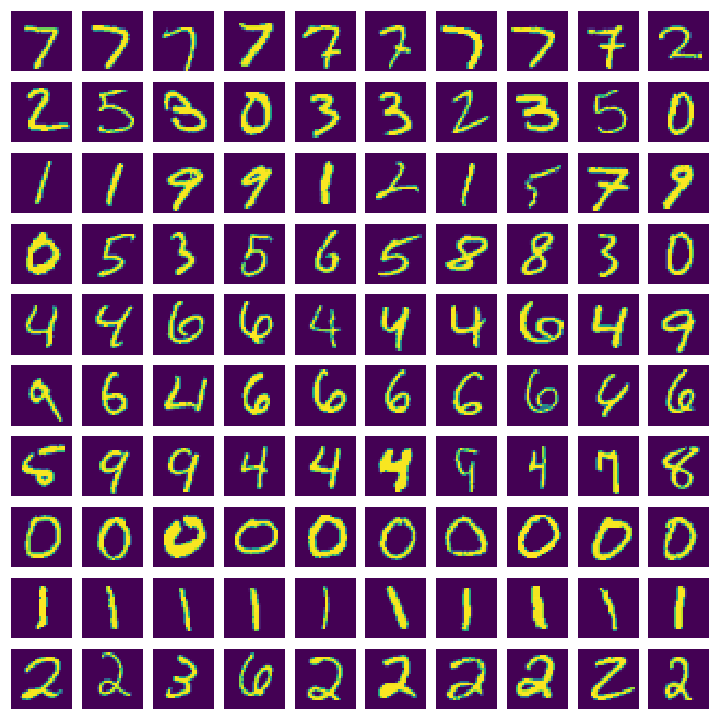
\includegraphics[width=\textwidth]{../../images/number_clustering_10_0norm.png}
                    \caption{Count of pixels that are non-zero in both images as similarity measure}
                    \label{fig:clustering_10_0norm}
                \end{subfigure}           
                \begin{subfigure}[b]{0.3\textwidth}
                    \centering
                    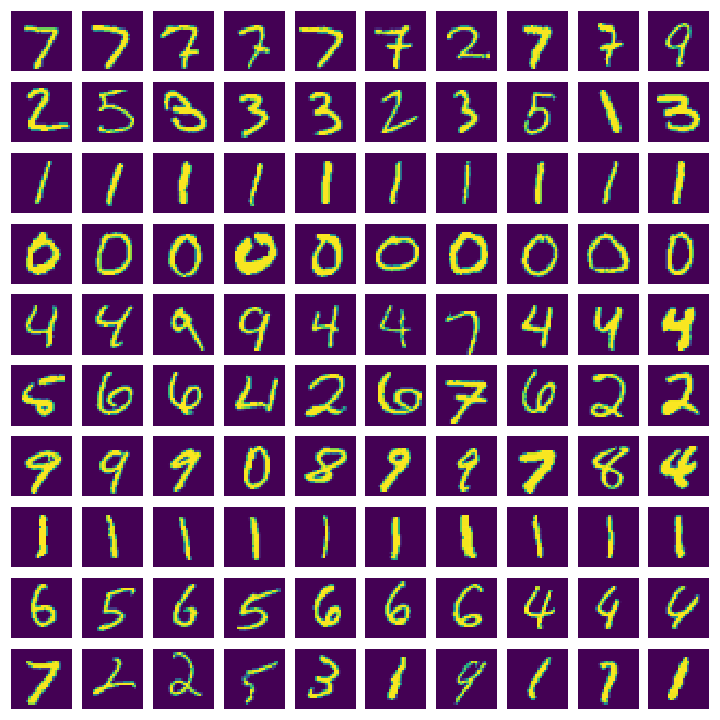
\includegraphics[width=\textwidth]{../../images/number_clustering_10_2norm.png}
                    \caption{Inverse of 2-norm of the difference vector between two images as similarity measure}
                    \label{fig:clustering_10_2norm}
                \end{subfigure}           
                \begin{subfigure}[b]{0.3\textwidth}
                    \centering
                    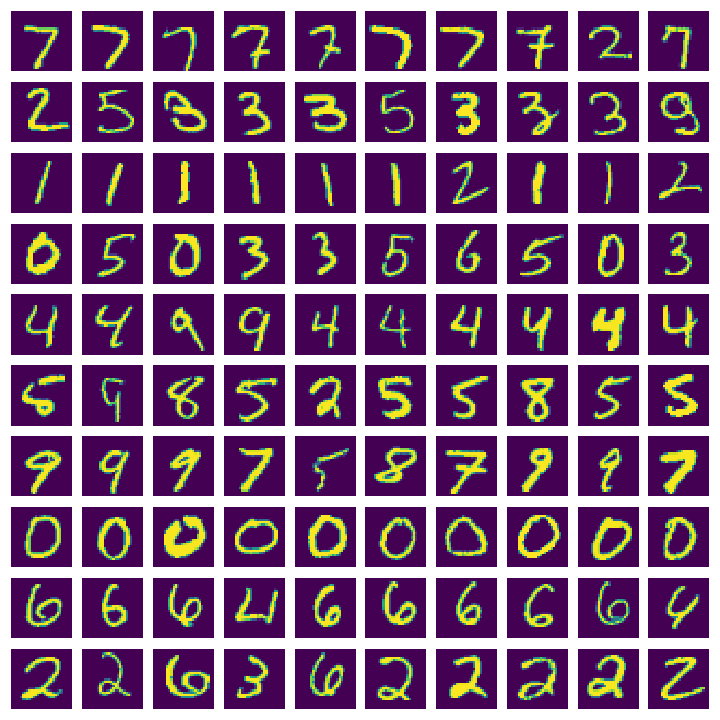
\includegraphics[width=\textwidth]{../../images/number_clustering_10_hamming.png}
                    \caption{Count of pixels that are zero or non-zero in both images as similarity measure}
                    \label{fig:clustering_10_hamming}
                \end{subfigure}           
            \end{center}
            \caption{2000 images from MNIST dataset were clustered into 10 clusters. In the above figure, each row of images represent a cluster and show the first 10 images in that cluster}
            \label{fig:mnist10ClusterImages}
        \end{figure}

        \begin{figure}[h]
            \begin{center}
                \begin{subfigure}[b]{0.3\textwidth}
                    \centering
                    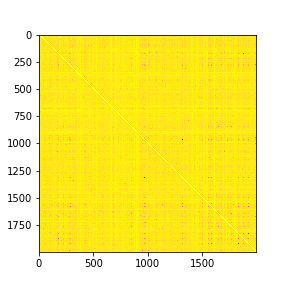
\includegraphics[width=\textwidth]{../../images/w_0norm.png}
                    \caption{Count of pixels that are non-zero in both images as similarity measure}
                    \label{fig:w_0norm}
                \end{subfigure}           
                \begin{subfigure}[b]{0.3\textwidth}
                    \centering
                    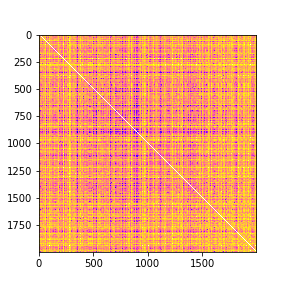
\includegraphics[width=\textwidth]{../../images/w_2norm.png}
                    \caption{Inverse of 2-norm of the difference vector between two images as similarity measure}
                    \label{fig:w_2norm}
                \end{subfigure}           
                \begin{subfigure}[b]{0.3\textwidth}
                    \centering
                    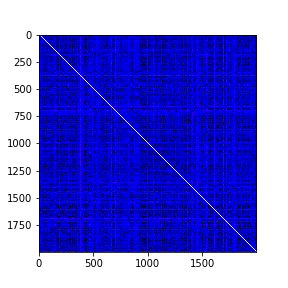
\includegraphics[width=\textwidth]{../../images/w_hamming.png}
                    \caption{Count of pixels that are zero or non-zero in both images as similarity measure}
                    \label{fig:w_hamming}
                \end{subfigure}           
            \end{center}
            \caption{Weighted adjecency matrix for 2000 images from MNIST dataset with similarity functions described under the images}
            \label{fig:mnistWImages}
        \end{figure}


        \begin{figure}[h]
            \begin{center}
                \begin{subfigure}[b]{0.4\textwidth}
                    \centering
                    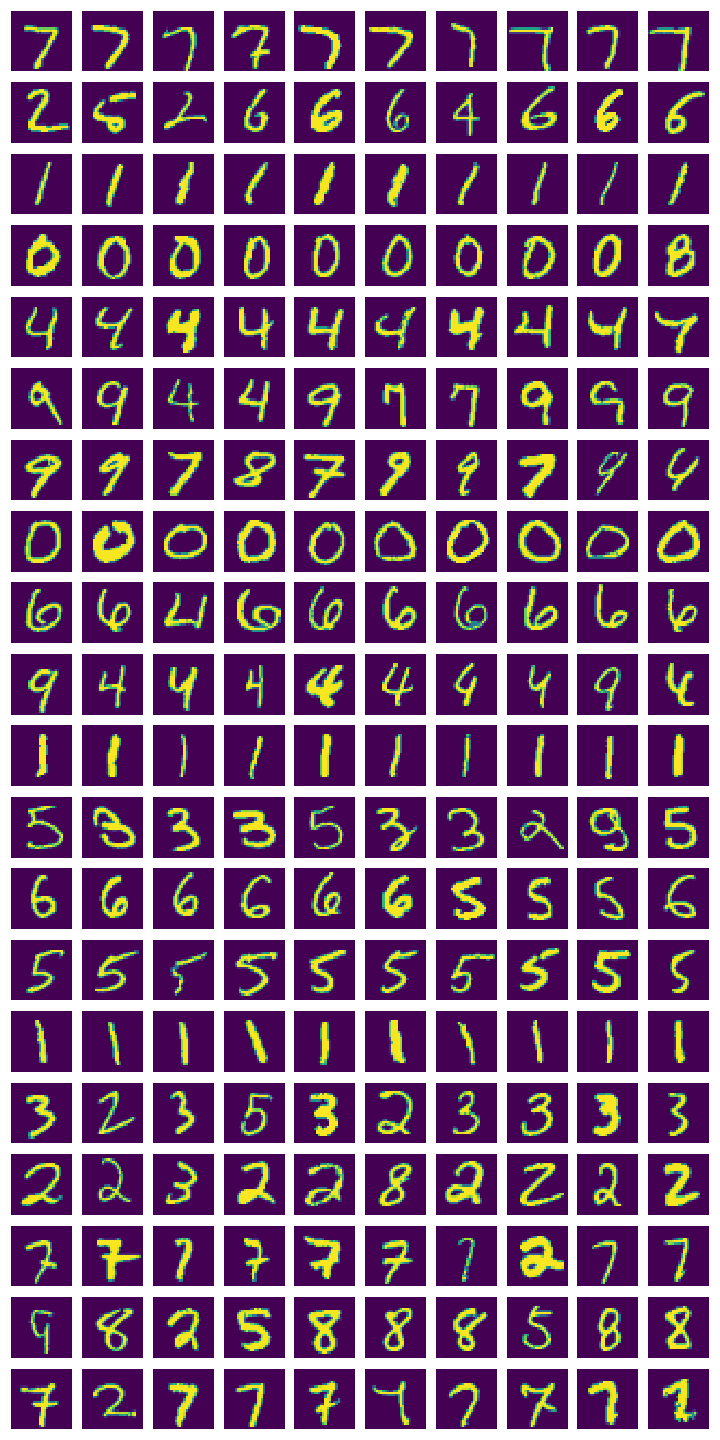
\includegraphics[width=\textwidth]{../../images/number_clustering.png}
                    \caption{Count of pixels that are non-zero in both images as similarity measure}
                    \label{fig:clustering_20_0norm}
                \end{subfigure}
                \begin{subfigure}[b]{0.4\textwidth}
                    \centering
                    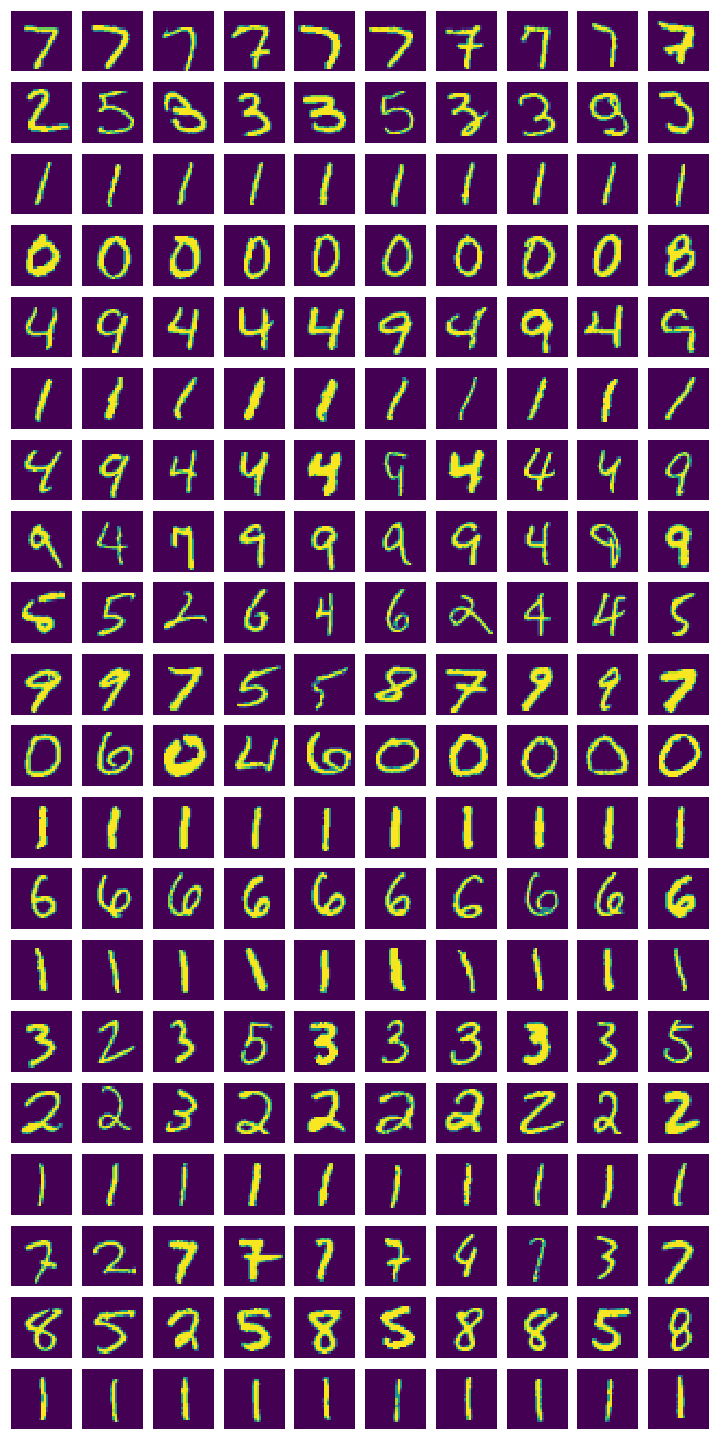
\includegraphics[width=\textwidth]{../../images/number_clustering_20_2norm.png}
                    \caption{Inverse of 2-norm of the difference vector between two images as similarity measure}
                    \label{fig:clustering_20_2norm}
                \end{subfigure}
            \end{center}
            \caption{2000 images from MNIST dataset were clustered into 20 clusters. In the above figure, each row of images represent a cluster and show the first 10 images in that cluster}
            \label{fig:mnistImages}
        \end{figure}

        
    \end{enumerate}
    
    
    \section{Practical considerations and challenges}

    While the algorithms are relatively simple to implement, there are some issues that arise in practice. 
    
    \subsection{Parameters and Tuning Considerations}
    The first consideration is the choice of similarity function. The effectiveness of the algorithm depends upon the similarity matrix $W$ which is defined by the similarity function. Although Gaussian similarity function $exp(-\norm{x_I - x_j}^2)/(2\sigma^2)$ is generally a reasonable choice in Euclidean space, the choice of similarity function would generally be guided by the domain of application. 

    Next would be the choice of similarity graph and its parameters. The type of graph ($k$-nearest neighbor, $\epsilon$-neighborhood, etc.) affects how the areas of different densities are treated. For example, a $k$-nearest neighbor graph may cause some points in a sparse cluster to be connected to a dense cluster or may break a high-density cluster into smaller clusters if $k$ is not chosen appropriately. Also for $\epsilon$ neighborhood graph, the choice of $\epsilon$ dictates the sparsity of the matrix. While sparse matrix would be desirable since use of eigensolvers can speed up the eigenvector calculation, it can also lead to loss of information and hence a balance must be achieved and choice of the parameters should be guided by the domain of application. 

    Choice of Laplacian is the next concern. Recall that the goal of clustering is two-fold, to minimize inter-cluster similarity or $cut(A,\bar{A})$, and maximize within-cluster similarity or $W(A,A)$. Both Ncut and RatioCut will achieve the first objective since they both have $cut(A,\bar{A})$ in the numerator. However, note that $W(A,A) = W(A,V) - W(A,\bar{A}) = vol(A) - cut(A,\bar{A})$. This means that within-cluster similarity is maximized when $cut(A,\bar{A})$ is minimized and $vol(A)$ is maximized. This is where Ncut outperforms RatioCut since it has $vol(A)$ in the denominator. Hence $L_{rw}$ is generally a good choice.

    \subsection{Challenges}

    The following are the challenges that frequently arise in practice. 

    Computing eigenvectors can be an expensive task, particularly if the matrix is large and dense. Fortunately a properly chosen graph and parameter(s) (e.g. $k$ for $k$-means or $\epsilon$ for $\epsilon$ neighborhood), should lead to a sparse matrix, which, in turn, facilitates the choice of sparse eigensolvers and hence speed up the calculation. Additionally, the convergence speed depends upon spectral gap $\gamma_k = \abs{\lambda_k - \lambda_{k+1}}$. Hence scaling and shifting or methods like MAPS described in \cite{Lu2015AcceleratedAF} can be applied. 

    Next, challenge would be to choose the number of clusters. While the literature that describes the algorithms and their designs, usually takes the number of clusters, $k$, as input to the algorithms, frequently in practice, one needs to find the number of clusters that exist in a dataset. Since this is a general problem for all clustering algorithms, a variety of methods exist. Some methods use the ratio of within-cluster to inter-cluster similarity or distance as a measure of how good the clustering is, while other methods use a statistical calculation based on log-likelihood of data. Additionally, for spectral clustering, eigengap is an important heuristic. A good starting point is to choose $k$ such that $\lambda_1,\dots,\lambda_k$ are small but $\lambda_{k+1}$ is relatively large. However, the effectiveness of this technique depends on how well the clusters are differentiated.

    Finally, the $k$-means step itself can be expensive and in some cases, may not lead to ideal results based on the initial guess and/or the distribution of data points. Several attempts have been made to use other techniques of clustering. In \cite{Bottou95convergenceproperties}, the authors show that $k$-means is efficient and minimizes the quantization error, thus highlight the reasons why $k$-means has become the choice for clustering applications. 
    
    \section{Compressive Spectral Clustering}
    In Compressive Spectral Clustering \cite{tremblay-compressive-SC-16}, the authors propose an algorithm to sample $\mathcal{O}(\log(k))$ randomly filtered signals on the graph to serve as feature vectors instead of eigenvectors and by clustering random subset of $\mathcal{O}(k\log(k))$ nodes using random feature vectors and inferring the cluster label of all $N$ nodes. This algorithm speeds up the clustering process by reducing the dimensionality and hence, the size of the problem.

    As discussed above, for a graph with $k$ connected components, 0 is the eigenvalue with multiplicity $k$ and the corresponding eigenvectors would be the indicator vectors of the clusters, which would be orthogonal. Thus, the indicator vectors belong to $span\{U_k\}$. Perturbation theory says that for the general graph with slight perturbation to the ideal case, the first $k$ eigenvectors still belong to $span\{U_k\}$. Thus it should be possible to sample a smaller number of features and still have $k$-means identify the $k$ clusters correctly. 

    The algorithm for compressive spectral clustering is, however quite involved and is outlined briefly below. 

    \begin{itemize}
        \item First, to get the first $k$ eigenvectors,  
            \begin{itemize}
            \item Estimate the $k^{th}$ eigenvalue using eigen-counting techniques detailed in \cite{Di13efficientestimation} 
            \item Build polynomial estimation of the low-pass filter $H := h(L) = U h(\Lambda) U^T$ where $h({\Lambda})$ is the diagonal matrix with 1 on primary diagonal for the first $k$ rows/columns and 0 otherwise. $U$ here is the matrix is the eigenvectors of $L$. However, $L$ is not diagonalized, instead $Hx$ is approximated as $\sum_{l=0}^{p}\alpha_l L^{l}x$ by successive matrix-vector products with $L$.
            \end{itemize}
        \item  Generate $d$ random Gaussian signals $r_1,\dots, r_d$ with mean $0$ and variance $1/d$, Let $S = (r_1|r_2|\dots|r_d) \in \mathbb{R}^{N\times d}$
        \item Filter $S$ with $H$ and define for each node $i$, its feature vector $\bar{f}_i \in \mathbb{R}^d = \big[ (HS)^T \delta_i \big] / \norm{(HS)^T \delta_i} $
        \item Generate random sampling matrix $M\in \mathbb{R}^{n\times N}$ to keep $n=2k \log{k}$ features. 
        \item Run $k$-means on the reduced dataset with Euclidean vector distance to obtain $k$ reduced indicator vectors, one for each cluster. 
        \item Interpolate each reduced indicator vector to find the cluster assignment for each node on the graph.
    \end{itemize}

    \chapter{Intended Work}
    In practice quite frequently the number of clusters is not known. Hence a clustering method is repeatedly applied with an increasing number of clusters until the desired accuracy is reached. With spectral clustering, since the number of clusters depends on the number of eigenvectors used, the information from a prior step may be used in the subsequent step to avoid redundant work. For example, since the first $k$ eigenvectors and hence, eigenvalues are, known, we may be able to use this knowledge in, at least, providing bound on the next eigenvalue and use shift inverse power iteration. 

    Another possibility is to use Krylov subspace based methods. Although I do not have a clear path, Krylov-space methods are an attractive possibility for two reasons, one is that adding dimensions, i.e. subsequent basis vectors is simply a matrix-vector product and the second reason is that $L$ and $L_{sym}$ are symmetric and thus will lead to Lanczos method and tridiagonal instead of Hessenberg matrix. It may be possible to achieve clustering using Krylov subspace basis vectors, thus we may not need to compute the eigenvectors. 


    \appendix
    \chapter{Propositions related to Graph Laplacians}
    \begin{prop}(Properties of L) The matrix L satisfies:
        \begin{enumerate}
            \item for every vector $f \in \mathbb{R}^{n}$ we have $$ f_{T}Lf = \frac{1}{2}\sum_{i,j=1}^{n} w_{ij}(f_{i}-f_{j})^{2} $$
            \item L is symmetric and positive semi-definite
            \item The smallest eigenvalue of L is 0, the corresponding eigenvector is the constant vector $\mathbf{1}$
            \item L has $n$ non-negative, real-values eigenvalues $0=\lambda_{1} \le \lambda_{2} \le \cdots \le \lambda_{n}$
        \end{enumerate}
    \end{prop}
    \textit{Proof:}
    \begin{enumerate}
        \item  By definition of $d_{j} = \sum_{i=1}^{n}w_{ij}$
        \begin{align*}
        f'Lf & = f'Df - f'Wf = \sum_{i=1}^{n}d_{i}f_{i}^{2} -  \sum_{i,j=1}^{n}f_{i}f_{j}w_{ij}\\
        & = \frac{1}{2}\bigg(\sum_{i=1}^{n}d_{i}f_{i}^{2} -  2\sum_{i,j=1}^{n}f_{i}f_{j}w_{ij} + \sum_{i=j}^{n}d_{j}f_{j}^{2}\bigg)\\
        & = \frac{1}{2}\sum_{i,j=1}^{n}w_{ij}(f_{i}-f_{j})^{2}
        \end{align*}
        \item Since $W$ and $D$ are symmetric $L = D-W$ is still symmetric. By result of part (a), since $w_{ij} \ge 0$ and $(f_{i}-f_{j})^{2} \ge 0$, $f'Lf \ge 0$, hence $L$ is symmetric and positive semi-definite
        \item See proposition 2
        \item Since $L$ is symmetric, all its eigenvalues are real. Also by part (c), the smallest eigenvalue is 0, 
    \end{enumerate}

    Note that the unnormalized graph Laplacian does not depend on the diagonal elements of $W$. $d_{ii} = \sum_{j=1}^{n}w_{ij}$, hence the diagonal elements are canceled by $d_{ii}$ and the self-edges do not change the Laplacian. \\
    
    \begin{prop}
        (Number of connected components and the spectrum of $L$) Let $G$ be an undirected graph with non-negative weights. Then the multiplicity $k$ of the eigenvalue $0$ of $L$ equals the number of connected components $A_{1},\cdots,A_{k}$ in the graph. The eigenspace of eigenvalue $0$ is spanned by the indicator vectors $\mathbf{1}_{A_{1}},\cdots,\mathbf{1}_{A_{k}}$ of those components.				
    \end{prop}
    \textit{Proof:}
    Starting with $k=1$, i.e. graph is fully connected. Assume that $f$ is the eigenvector with eigenvalue $0$. Then,
    $$ 0 = f'Lf = \sum_{i,j=1}^{n}w_{ij}(f_{i}-f_{j})^{2} \implies f_{i} - f_{j}=0 \hspace{10pt}[\because w_{ij} > 0]$$
    
    Since we assumed a fully connected graph, $f$ has to be constant for the above argument to be true for any vertex in the connected component. Hence the vector $\textbf{1}$, which is the indicator vector of the component is an eigenvector corresponding to eigenvalue $0$. 
    
    Now, for $k>1$, we can easily rearrange the vertices in the matrix to put all the vertices of a connected component together. This would cause the matrix $L$ to be a block diagonal matrix. For each of these blocks, or components, the respective indicator vector is an eigenvector with eigenvalue 0. Thus the Matrix $L$ has eigenvalue $0$ with multiplicity equal to the number of components and the corresponding eigenvectors would be the indicator vectors of those components. 
    $ $\\

    \begin{prop}
        (Properties of $L_{sym}$ and $L_{rw}$)
        \begin{enumerate}
            \item
            For every $f\in\mathbb{R}^{n}$
            $$ f'L_{sym}f = \frac{1}{2}\sum_{i,j=1}^{n}w_{ij}\bigg(\frac{f_{i}}{\sqrt{d_{i}}}-\frac{f_{j}}{\sqrt{d_{j}}}\bigg)^{2} $$
            \item $\lambda$ is an eigenvalue of $L_{rw}$ with eigenvector $u$ iff $\lambda$ is an eigenvalue of $L_{sym}$ with eigenvector $w=D^{1/2}u$.
            \item $\lambda$ is an eigenvalue of $L_{rw}$ with eigenvector $u$ iff $\lambda$ and $u$ solve the generalized eigenproblem $Lu=\lambda Du$
            \item $0$ is an eigenvalue of $L_{rw}$ with the constant one vector $\mathbf{1}$ as eigenvector. $0$ is an eigenvalue of $L_{sym}$ with eigenvector $D^{1/2}\mathbf{1}$
            \item $L_{sym}$ and $L_{rw}$ are positive semi-definite and have $n$ non-negative real-valued eigenvalues $0=\lambda_{1} \le \lambda_{2} \le \cdots \le \lambda_{n}$
        \end{enumerate}
    \end{prop}
    \textit{Proof:}
    \begin{enumerate}
        \item This can be proved similar to part 1 of proposition 1. 
        \item Assume $\lambda$ is an eigenvalue of $L_{sym}$ with eigenvector $w=D^{1/2}u$. 
        \begin{align*}
        L_{sym}D^{1/2}u &= \lambda D^{1/2}u \\
        \implies  D^{-1/2}LD^{-1/2}D^{1/2}u &= \lambda D^{1/2}u \\
        \implies D^{-1}Lu &= \lambda u \hspace{10pt}[\text{left multiplying with } D^{-1/2}] \\
        \implies L_{rw}u &= \lambda u
        \end{align*}
        In other words, u is eigenvector of $L_{rw}$. To prove the other direction, apply the above steps in reverse order.
        \item This can be proven in similar manner to above by left multiplying the generalized eigenproblem $Lu = \lambda Du$ with $D^{-1}$
        \item $L_{rw}\mathbf{1} = (I-D^{-1}W)\mathbf{1} = \mathbf{1}-\mathbf{1} = 0$.\\ The above is true because $d_{i} = \sum_{j=1}^{n}wij \implies \big(D^{-1}W)\mathbf{1}\big)_{i} = \sum_{j=1}^{n}\frac{w_{ij}}{d_{i}}$, since $\mathbf{1}$ is the indicator vector. Then using part (b) leads to the second statement of this property. 
        \item The first part (for $L_{sum}$) can be proved from part (a), similar to Proposition 1. Part 2 essentially states that $L_{sym}$ and $L_{rw}$ have the same eigenvalues, hence second statement is also proven.
    \end{enumerate}					

    \begin{prop}
        (Number of connected components and spectra of $L_{sym}$ and $L_{rw}$) Let $G$ be an undirected graph with non-negative weights. Then the multiplicity $k$ of the eigenvalue $0$ of both $L_{sym}$ and $L_{rw}$ equals to the number of connected components $A_{1},\cdots,A_{k}$ in the graph. for $L_{rw}$, the eigenspace of $0$ is spanned by the indicator vectors $\mathbf{1_{A_{i}}}$ of these components. for $L_{sym}$ the eigenspace of $0$ is spanned by $D^{1/2}\mathbf{1_{A_{i}}}$
    \end{prop}
    \textit{Proof:} The proof of this is analogous to that of proposition 2, but using proposition 3.


	\nocite{govl:96, parlet:98,stsu:90,gene:2018}
	
	\thispagestyle{fancy}
	\bibliographystyle{unsrt}
	\bibliography{long_string, Mybib} 
	
\end{document}